\chapter{The Quest for Meaning in Video}
\label{ch:quest}

\section{Introduction} % (fold)
\label{sec:introduction}

% start intro: consider example of a video segment; indicate how its easy for humans to `understand' the content on multiple levels
Interpreting moving images is not a hard task. The medium film is often described as `dictatorial' because of the way the audience is immersed in a multi-modal experience controlled by the creators. We can sit back and relax, passively taking in the presented information without much effort. A similar ease is reflected in our use of the word `couch potato' to describe the passive role of television audiences. Watching film or video gives us almost immediate access to a wide range of information about what is presented on screen. We recognise objects on screen and understand words that spoken in a language we know. We are also quick to infer a larger picture around the things we perceive, like personality traits of characters on screen or our emotional stance towards them. While most of these things happen extremely quickly and seemingly automatically to us humans, computers often have a hard time even starting to perceive a visual representation of an object.

% explain how computers are having difficulties. in recognition, spatio/temporal segmentation (figure ground), qualitative evaluations are even more difficult.
When we attend to visual content depicting parts of the world around us, we can't help ourselves from seeing its parts as separate entities. We recognise objects as if they stand out from their background even though they are simply patterns of colours on a two dimensional surface. To a computer, tasks like object segmentation and recognition are hard because visual information needs to be interpreted in some form of sequential processing. Digitally, images are usually represented by collections of numbers indicating local intensities (e.g. brightness) at the different points that make up the image. How to calculate from this information, which objects are present, and what other concepts can be assigned to an image is studied in the field of computer vision. Although recent years have seen important advances in the use of high-level semantical concepts in tasks like video concept detection and concept-based video retrieval \cite{Snoek:2009dq, Snoek:jf, Worring:2007vm, Chang:2008wh}, computational methods commonly have difficulties in performing both reliably and generally.

% from world -> representation -> concepts
To better understand what is going on in the interpretation of visual content by both humans and computers, it helps to model it as a process from start to end. Figure \ref{fig:understanding_visuals} shows in a high-level model how objects in the world are sensed and consequently rendered in a visual representation. We can think of this process taking place when we photograph a car and end up with a picture of that car as a result. When the representation of an object is next interpreted by someone, we can think of this person as establishing semantical concepts relating to aspects of the depiction. A situation to which we can map this part of the model would be someone looking at the picture and recognising the car.

\begin{figure}[htbp]
  \centering
    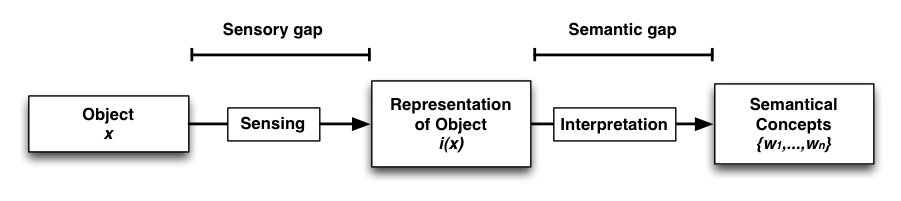
\includegraphics[width=.8\textwidth]{understanding_visuals}
  \caption{A high level model of the interpretation of visual media content}
  \label{fig:understanding_visuals}
\end{figure}

% first problem: sensory gap
A first source of complication in the way from object to its interpretation, is the sensory gap, described by Smeulders et al. as:

\begin{quote}
  ``The sensory gap is the gap between the object in the world and the information in a (computational) description derived from a recording of that scene.''\cite{Smeulders:2000tx}
\end{quote}

% second problem: semantic gap
The second way meaningful interpretation of visual content is hampered, is the semantic gap that lies between a digital representation and the conceptual interpretation we address to it. Snoek and Worring adapt the origianal definition from \cite{Smeulders:2000tx} to specifically fit the medium video:

\begin{quote}
  ``The lack of correspondence between the low-level features that machines extract from video and the high-level conceptual interpretations a human gives to the data in a given situation.''
\end{quote}

% scope of this chapter
Because of the often elusive character of concepts like meaning and understanding, we take care to keep our intentions for this chapter humble. The intension is not to give an accurate explanation of daunting concepts like meaning or semantics, nor is it to give an accurate account of the diverse work on the relationship between signifier and signified in the field of semiotics. This first chapter is meant to briefly introduce the difficulties that current computational methods have in arriving at a meaningful interpretation of visual content. To this purpose we formulate a framework of computational analyses of meaning that serves to establish terminology to work with in the remainder of this work, rather than to make claims about the deeper functioning of human understanding or signifying systems.


% section introduction (end)



\section{The Need for Labeling}

Whereas textual data can be searched relatively easily because of its symbolic nature, this is more difficult for video. Because visual data on it's own provides little machine-readable handles to search for, repositories of multimedia content need to be indexed with symbolic labels to enable search and retrieval. 


\subsection{Human Labelling}

\subsection{Machine Labelling}


\section{The Semantic Gap}


\section{Computationally Narrowing the Gap}

\subsection{Supervised Concept Learning}

The paradigm most in use for the detection of concepts in video is supervised learning. In a supervised machine learning task, one learns the relation between a collection of input values and a smaller set of output values. A relation between inputs and outputs is learned by presenting a large number of training examples as input along with their respective output values. For video concept detection, input values are usually a collection of features representing different aspects of the video while outputs code for the concept that is known to be present. 

Although detectors can be trained to learn to detect patters of multiple concepts, usually a separate concept detectors are trained for distinct concepts. By applying multiple detectors on an previously unseen input instance, multiple concepts can be detected.

\subsection{Video Feature Extraction}

\subsubsection{Meaning in Visual Features}

Visual features are extracted both locally at the level of regions and pixels and globally at the level of frames.

\paragraph{Color}

\paragraph{Texture}

\paragraph{Shape}

\subsubsection{Meaning in other Modalities}
The use of audio and text for extraction of features.

[Telop-on-demand: Video structuring and retrieval based on text recognition]\cite{Kuwano:2000wy}
[Addressing the Challenge of Visual Information Access from Digital Image and Video Libraries]\cite{Christel:2005td}

\subsection{Meaning in Structure}


[cite bordwell \& Thompson: analysis of context dependency]
[link to narratives and storytelling]
% hypervideo as form of 1 narrative 2 navigation, link to database documentary
[HyperCafe: Narrative and Aesthetic Properties of Hypervideo \cite{Sawhney:1996tk}]

\subsubsection{Spatial Structure}
\subsubsection{Temporal Structure}




\section{Interactive Storytelling: From database to data-based}
\label{ch:storytelling}
\subsection{Symbolic approaches}
\label{sec:symbolic}

\cite{Vilmos:2011wv,RodrigoLaiolaGuimaraes:2011tl,Ursu:2009gc}

\subsection{Statistic approaches}
\label{sec:statistic}

\subsection{Remixing}

The reconfiguration of smaller units that carry meaning within themselves is common practice for textual media such as blogs, where it is easy to quote part of  another author`s writing in a new post [ref]. 

It needs to be said that some reconfiguration of videos is taking place, but even though it often concerns content that was originally sourced online, much of the creative act of remixing happens offline.


\subsection{Taking the remix online}

examples like: Aaron Koblin (johnny cash project, exquisite corps, etc)

there is even word of a true remix culture.

the availability of multimedia content via the internet has meant a surge in 


\section{Computational Difficulties}

% problem is that no CV algorithms perform reliable AND generally

% the problem of acquiring labelled data for ML approaches
% problem of keeping ML techniques up to date in a dynamical environment where new content is added every minute (and a lot of it as we will see when we discuss user generated online video)





